\chapter{How to run a TINIBA test case}

CODE:

\textcolor{darkgreen}{``drakgreen'' for the TINIBA$^{\reg}$ commands}

\textcolor{blue}{``blue'' for the input}

\textcolor{orange}{``orange'' for the Linux commands}

\verb= verbatim for directories or files=

\textcolor{gray}{``gray'' for output}

\verb= i.e. = is for examples\\

\centerline{General Considerations}
\begin{itemize}
\item The same version of \verb=abinit= is runed in all platforms. If
  a new version is needed, just compile it, and let everybody
  know. Include this in \verb=utils/version-abinit.txt= (see \ref{av}).

\item There are three switches, one for the Xeons, one for the Quads
  and one for the Hexas. Thus is convenient to chose only one platform
  for the whole run, at least for the SCF cycle. This would take
  advantage of doing the \verb=mpi= and \verb=rcp= over the
  \verb=myrinet= or \verb=infiniband= switches.
\item \verb=ssh= to any of the \verb=xeon (node01-32)=, \verb=itanium01-04=,
  \verb=quad01-14= or \verb=hexa1-36= platforms. Then, \verb=cd= to the
  corresponding \verb=/home=, and work from there.
\item The RAID system has the following storage HD's\\
 \verb=/homea/ /homeb/ /homee/ /homeib/ /homen/ /homeu/=\\
where each user must store the work, once finished running in the cluster. 
\item It is very convenient to call the working directory with a
name that relates to the case you are working with. 
\item Since the SCF uses the parallelized version of \verb=abinit= is
  better to use only one platform for this cycle.
%\item \textcolor{red}{If the SCF cycle will be done in the}
%  \verb=QUADS=, 
%\textcolor{red}{it's better to work in the node} \verb=quad01:/homeib/$USER/=$\ldots$
\item If running in the \verb=quads= work in \verb=/homeib/=
and for the SCF cylce use at least
one \verb=quad01= in \verb=.machines_scf.original=.
\item The matrix elements could be calculated in the three plataforms,
  although for copying the wave function is much faster if it is done
  through the switches.  

\end{itemize}

The example is a slab of 6 layers mimicking Si(111):As with no spin-orbit
coupling. 
\begin{enumerate}
\item \verb=$PWD > ssh [quad01,hexaN]= 

\item\textcolor{red}{If} \verb=quad01= 
\begin{itemize}
\item \verb=$PWD > cd /homeib/user= 
\end{itemize}
\item\textcolor{red}{If} \verb=hexaN=
\begin{itemize}
\item \verb=$PWD > cd /home?/user/=  with ?=a,b,e,n,u 
\end{itemize}
\item 
\verb=$PWD >= \textcolor{darkgreen}{creatingTree.sh} \verb=si_as_6=
(optional)\\ \strut\hspace{.9cm}if so 
\begin{itemize}
\item \verb=$PWD >= \textcolor{orange}{cd} \verb=si_as_6/abinit-si_as_6/si_as_6/=\\else
\item \verb=$PWD >= \textcolor{orange}{cd} \verb=si_as_6=
\end{itemize}

The 
\verb=setUpAbinit_si_as_6.in=, \verb=si_as_6.xyz= and
\verb=.machines_*.original= files are found in
\verb=$TINIBA/examples/surface/nospin=. Copy these files to your
working directory and
\begin{itemize}
\item \textcolor{red}{WARNING}: The psudopotentials are in\\
\verb=$TINIBA/psp=\\
\textcolor{red}{Be sure that in that the path to them is correctly set
in}\\
 \verb=setUpAbinit_case.in= 
\item {\small Check that the input parameters are consistently
    taken. i.e. with/without spin-orbit coupling, etc.}
\item {\small Plot the coordinates to make sure they are correct.}
\item \verb=.machines_scf.original= 
for the SCF (\textcolor{red}{only chose one
 platform!})
\item \verb=.machines_pmn.original= for the matrix elements (\textcolor{red}{could chose mixed platforms})
\item \verb=.machines_latm.original= for the integrands (\textcolor{red}{only one CPU from any platform})
\item \verb=.machines_res.original= for the $\bfk$-integration
  (\textcolor{red}{chose as many CPU's, from any platform,
as tensor components to be calculated})
\end{itemize}
%\begin{enumerate}
\item \verb=$PWD > =\textcolor{darkgreen}{createRemoteDir.sh} (optional)
\begin{itemize}
\item Check that the chosen nodes are working:
\begin{itemize}
\item above removes all the nodes that  don't work or exist
\item You may want to remove above nodes from the \verb=*.original= files
\end{itemize}
\end{itemize}
\item{\small \verb=$PWD > =\textcolor{orange}{cluster\_exec -N}
   \textcolor{blue}{ALL} \textcolor{orange}{ps -u} \textcolor{blue}{username}
}
\begin{itemize}
\item {\small run in \verb=medusa=.}
\item {\small So you can check that the nodes chosen are not being used by other user.}
\end{itemize}
% aqui voy
\item \verb=$PWD > =\textcolor{darkgreen}{abinitCheck.sh} \textcolor{blue}{1} 
\item \verb=$PWD > =\textcolor{darkgreen}{abinitCheck.sh} \textcolor{blue}{2} 
\begin{itemize}
\item \textcolor{red}{Surface Calculations}: If the slab is
  centrosymmetric, responses like  Surface SHG would be identically
  zero. To get the correct surface response use\\
$\bullet$\verb=odd_rank.sh=\\
This shell takes the original centrosymmetric \verb=case.xyz=, adds a
small part to the $z$-coordinate of the bottom surface atom(s), so the
structure is non-centrosymmetric. 
Then, \verb=abinit_check.sh= is run with both options, so the
\verb=sym.d= file does not has inversion symmetry.  
The coordinates are reset to the original centrosymmetric \verb=case.xyz=.  
%so run_all.sh can be properly run for and odd-rank tensor surface response
\item Check for the total memory needed and be sure that it fits in the RAM memory:\\
\textcolor{gray}{This job should need less than\hfill ? Mbytes of memory}
\end{itemize}
\item \verb=$PWD > =\textcolor{darkgreen}{rklist.sh}
\textcolor{blue}{ $N_x$ $N_y$ $N_z$} [\textcolor{blue}{abinit} or \textcolor{blue}{wine2k}]
\begin{itemize}

\item {\small $N_i$ must be odd.}
\item {\small If in real space $L_x=n\times L_y$ take
$N_y= n\times N_x$.}
\item {\small For a surface take $N_z=2$.}
\item 
\textcolor{gray}{Do you want to add inversion? (1=yes, 0=no)}

This inversion is the time-reversal symmetry. If your case has
it answer \textcolor{blue}{1} 
otherwise \textcolor{blue}{0} 

\item{\small \verb=i.e. $PWD > =\textcolor{darkgreen}{rklist.sh}
\textcolor{blue}{ 19 19 2 abinit}

This generates 64 $N_k$-points in the IBZ.
}
\end{itemize}
\item \verb=$PWD > =\textcolor{darkgreen}{rlayer.sh} (Skip for Bulk a Calculation)
\begin{itemize}
\item Used to generate the layers of the slab
\item Follow instructions
\item Plot to confirm that the layers are ok:\\
\verb=gnuplot> p 'case.xyz' u 1:3 w lp=\\
\verb=gnuplot> load 'front.layers.xy'=\\
\verb=gnuplot> load 'back.layers.xy'=
\item \verb=layers.d= is the file with the layers to be calculated.  
\item To select any given set of layers\\ 
\verb=$PWD > chose_layers.sh=
\begin{itemize}
\item Follow instructions
\item This is convenient in order to speed
 up the calculation for slabs with many
 layers so one chooses only a few important layers. 
\item The original layers are kept in \verb=layers.d.original=
\end{itemize}
\end{itemize}
\item \verb=$PWD > =\textcolor{darkgreen}{run\_tiniba.sh}
 \textcolor{darkgreen}{-r} \textcolor{blue}{setkp} 
 \textcolor{darkgreen}{-k} \textcolor{blue}{$N_k$} 
 \textcolor{darkgreen}{-g} \textcolor{blue}{$w_I$} 
 \textcolor{darkgreen}{-G} \textcolor{blue}{$w_Q$} 
\begin{itemize}
%\item \verb=RUN==\verb=tiniba_run.sh= a  la BMS\\
%\verb=RUN==\verb=runBULK.sh= a  la Cabellos
\item This distributes $N_k$ points in the nodes given in
  \verb=.machines_pmn.original=
\item It chooses the nodes that are working and for the \verb=quads=
  and \verb=hexas= the ones
  that have \verb=infiniband= as well
\item where $w_{I,Q}$ are the weights for how fast are the Itanium and Quad processors with respect to the Xeon processors.
\textcolor{red}{Since it is better to run in only one platform, this
  is irrelevant, and we may delete it altogether in a future version
  of TINIBA$^{\reg}$
}
\item
 \verb=i.e. $PWD > =\textcolor{darkgreen}{run\_tiniba.sh}
\textcolor{darkgreen}{-r} \textcolor{blue}{setkp} 
\textcolor{darkgreen}{-k} \textcolor{blue}{64} 
\textcolor{darkgreen}{-g} \textcolor{blue}{2} 
\textcolor{darkgreen}{-G} \textcolor{blue}{4} 

\item \textcolor{gray}{1=Choose another weight or
    2=Exit to run the full script}\\answer accordingly
\end{itemize}
\newpage
\item 
 \verb=$PWD > =\textcolor{darkgreen}{run\_tiniba.sh}
\textcolor{darkgreen}{-r} \textcolor{blue}{run} 
\textcolor{darkgreen}{-k} \textcolor{blue}{$N_k$} 
\textcolor{darkgreen}{-N} \textcolor{blue}{$N_{\mathrm{Layer}}$} 
\textcolor{darkgreen}{-x} [s-\textcolor{blue}{1} or
p-\textcolor{blue}{2}] \textcolor{blue}{options:}  
\begin{verbatim}
   -w      Wave function(k)
   -m      rho(z) for a set of k-points in case.klist_rho
   -e      Energies E_{m}(k)
   -p      Momentum Matrix Elements p_{mn}(k), includes m=n
   -d      Layered ndot Matrix Elements rho_{cc'}(k) 
   -c      Layered Momentum Matrix Elements calp_{mn}(k)
   -l      Layered Diagonal Momentum Matrix Elements calp_{mm}(k)
   -s      Spin Matrix Elements S_{cc'}(k)
   -n      Layered Spin Matrix Elements calS_{cc'}(k)
   -b      bypass WF checkup (Never use on first run)
\end{verbatim}
where
\begin{itemize}
\item \verb=-k Nk=: is the number of $\bfk$-points or \verb=rho= for
the  -m option
\item \verb=-N N_Layer=: is the number of
layers ($\geq 0$) %or \verb=half-slab= or \verb=bulk=
\item \verb=-x [s-1,p-2]= runs the SCF in {\it s}erial-1 or {\it p}arallel-2 (\textcolor{red}{recommended})
\item Besides \verb=-w= 
any option \textcolor{red}{{\it includes}} the
   calculation of the wave function
\end{itemize}


\textcolor{red}{{\it WARNING}} don't run using options 
\verb=-c, -l or -n= simultaneoulsy!

\item Tips
\begin{itemize}
\item Run in a separate sequence. i.e.:
  \verb=-w= $\to$   \verb=-e -p= $\to$   any other one option.
\item Use the option \verb=-b= after second run, just to be sure that
  the \verb=WF= file was correctly copied. 
\item The file \verb=rvarios.sh= is a shell with all the steps to
  perform a {\it whole enchilada} calculation including the response
  functions. Get one from \verb=$TINIBA/examples/rvarios.sh= and
  modify it {\it ad libitum}.
\item Other \verb=rvarios-shg.sh= file for SHG to
  perform a {\it whole enchilada} calculation is at
 \verb=$TINIBA/examples/rvarios-shg.sh=.
  Modify it {\it ad libitum}.
\item run with\\ \verb=> nohup rvarios.sh=\\
Then kill the terminal so
  \verb=nohup= works correctly.
\item To run {\it without} coherences for the spin injection go to\\ 
\verb=$TINIBA/latm/SRC_1setinput/integrands.f90=\\
comment/uncomment the corresponding lines (look for {\it without}),
compile, rename the response for $\zeta$ and $\xi$ in\\
 \verb=$TINIBA/utils/responses.txt=\\
and run \verb=all_responses.sh=. Then, undo the changes!  
\end{itemize}

\item LDA Energy Gap and Scissors correction\\
To calculate the LDA gap and the scissors correction run and follow instructions
\begin{itemize}
\item \verb=gap_correction.sh=
\end{itemize}
\item Monitors:
\begin{itemize}
\item To monitor the status of the run

$\bullet$ \verb=culster_exec -N ALL 'ps -u user'=

\item To monitor the calculation time and status of the matrix
  elements use:

$\bullet$ \textcolor{darkgreen}{ontoi.sh}

\end{itemize}

\item If the SCF doesn't run, before you tray again, do
\begin{itemize}
\item\verb=$PWD > =\textcolor{darkgreen}{run\_tiniba.sh -r} \textcolor{blue}{erasescf}
\end{itemize}

\begin{figure}[t]
\begin{center}
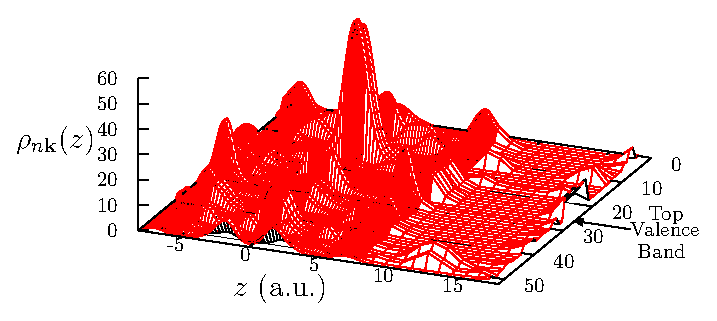
\includegraphics[scale=1.0]{plots/3drho}
\end{center}
\caption{$\rho_{n\bfk}(z)$ for the Si(111)As surface of the example
  calcuated with spin-orbit interaction.
}
\label{figrho}
\end{figure}

\item Integrated density  $\rho_{n\bfk}(z)=\int dx\int  dy\,|\psi_{n\bfk}(\bfr)|^2$ (see Fig. \ref{figrho})

\begin{itemize}
\item
 write or generate \verb=case.klist_rho= with the
 $\bfk$-points where it
needs to be evaluated, typical the $\Gamma$ point and some other few
points of maximum
symmetry. \textcolor{red}{Modify}\verb=.machines_pmn= such that the
number of $\bfk$-points is the same as the number of CPU's.
\item run with option \verb=-m= and follow instructions.
\end{itemize}
\item After you are done with the calculation erase as follows:
\begin{itemize}
\item\verb=$PWD > =\textcolor{darkgreen}{run\_tiniba.sh -r} \textcolor{blue}{erase}

to erase the files in all the nodes.

\item\verb=$PWD > =\textcolor{darkgreen}{run\_tiniba.sh -r} \textcolor{blue}{erasescf}

to erase the SCF calculation.\textcolor{red}{Warning: this erases the wave-function and may
 be better to keep it for future calculations, perhaps in a back-up HD}.

\end{itemize}

\end{enumerate}

\section{Benchmark Test}

Above example is run automatically by using and following the
instructions of\\
$\bullet$ \verb=$PWD >$TINIBA/utils/run-whole-enchilada-surface.sh=\\
where the output ought to be compared with benchmark results in order
to check that TINIBA$^{\reg}$ is working correctly.

However the calculation of $\chi^{\rmx\rmy\rmz}(2\go)$ for GaAs is a
better benchmark, since it is more sensitive to all the ingredients of
the calculation. It is run with\\
$\bullet$ \verb=$PWD >$TINIBA/utils/run-whole-enchilada-bulk.sh=\\
